\begin{figure}
    \centering
\begin{knitrout}
\definecolor{shadecolor}{rgb}{0.969, 0.969, 0.969}\color{fgcolor}
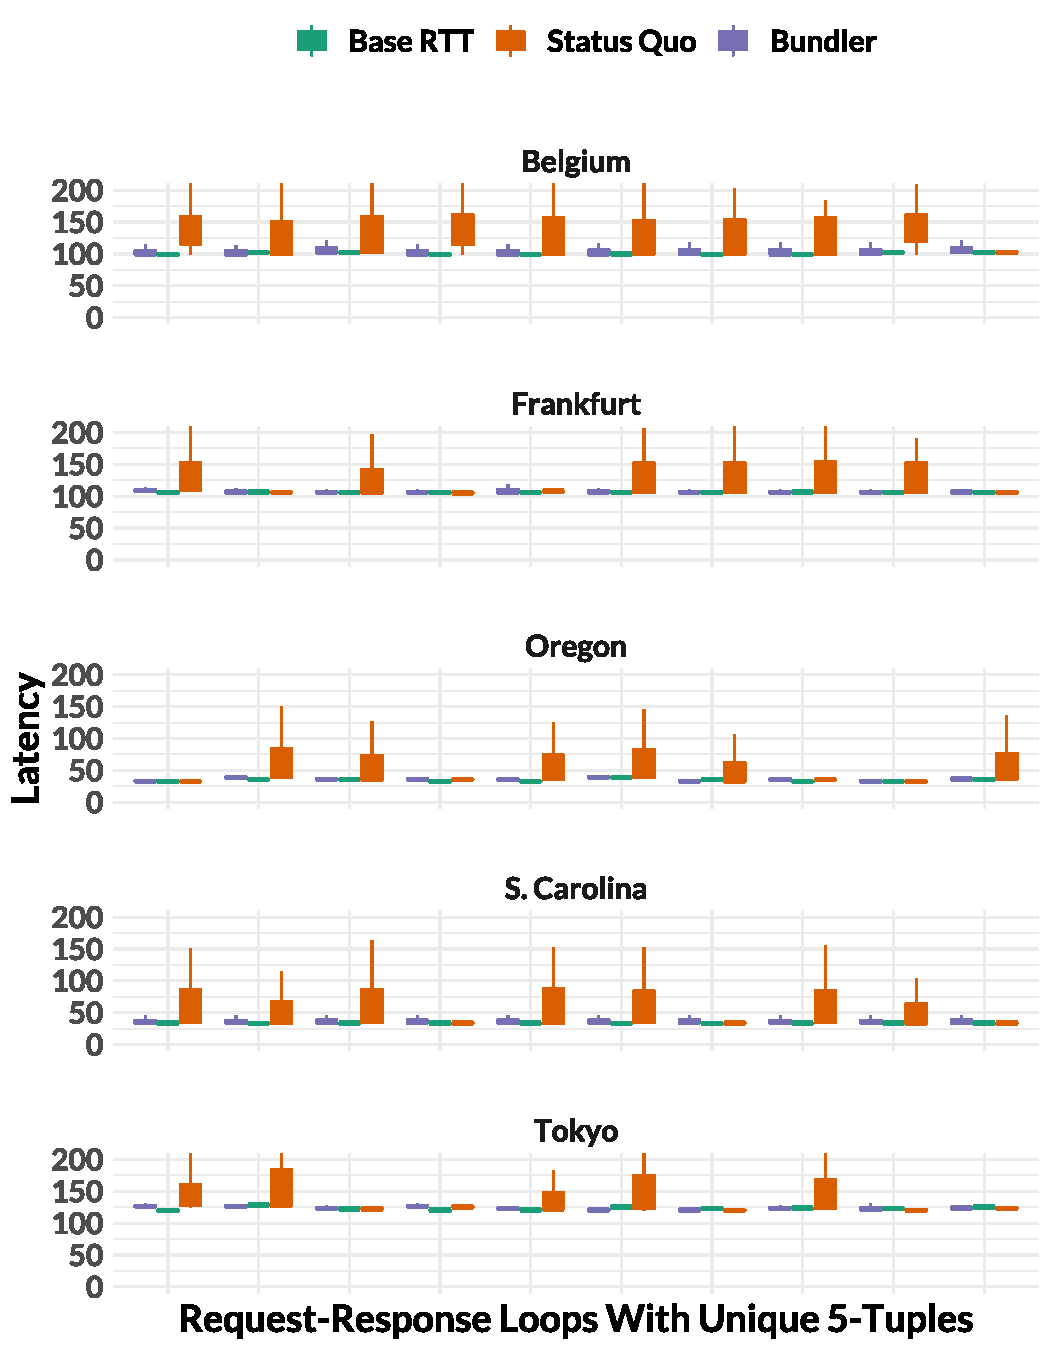
\includegraphics[width=\maxwidth]{figure/eval:realworld-1} 

\end{knitrout}
    \caption{On 5 real-Internet paths from the GCP datacenter in Iowa, \name achieves close to the Base RTT for latency-sensitive traffic. Each bar depicts an individual 5-tuple. On some paths, load-balancing in the Internet causes only some 5-tuples to experience queueing. \name offers scheduling for those paths.}
    \label{fig:eval:realworld}
\end{figure}
%\newcommand{\overviewBenefitsBundlerMedianImprovement}{round(100*(1-(overview_benefits_bundler_results[1] / overview_benefits_baseline_results[1])), 0)\%\xspace}
